\documentclass[aspectratio=1610,12pt]{beamer}
\definecolor{spoiler}{gray}{0.55}

\usepackage[utf8x]{inputenc}
\usepackage[russian]{babel}
\usepackage{xcolor,wrapfig,sistyle}

\usetheme{Berlin}
\usecolortheme{dolphin}

\definecolor{hardgreen}{RGB}{25,125,100}
\definecolor{softgreen}{RGB}{80,175,150}

\setbeamercolor{structure}{fg=hardgreen}
\setbeamercolor{subsection in head/foot}{bg=softgreen,fg=white}
\setbeamercolor{section in head/foot}{bg=hardgreen,fg=white}

\def\nagrslide#1#2#3{
	\fram{Сейчас награждаются}{\Large
		\begin{center}\begin{tabular}{|c|c|}
			\hline
			\ \ $\vphantom{\sum\limits_1^1}$ #1 класс\ \ \ &
			\ \ #2 вариант\ \ \ \\
			\hline 
			\multicolumn{2}{|c|}{$\vphantom{\sum\limits_1^1}$
				#3 степени} \\
			\hline
		\end{tabular}\end{center}}
}

\title[«Математика НОН-СТОП — 2018», решения избранных задач]
	{\bfseries Церемония награждения \\
		победителей и призёров Олимпиады \\
		«Математика НОН-СТОП — 2018»}

\author[Оргкомитет Олимпиады]
	{Лаборатория непрерывного \\ математического образования}

\institute[\textcolor{white}{«Время науки», ЛНМО, СПбАППО}]{}

\date{21 апреля 2018}

\def\fram#1#2{\begin{frame}\frametitle{\bf #1}#2\end{frame}}
\def\scolon{\rlap{,}\raisebox{0.8ex}{,} }
\def\mitem{\medskip\item}

\begin{document}
\begin{frame}\titlepage\end{frame}

\section[Награждение]{Awards}
\def\nagrgroup#1#2{
	\nagrslide{#1}{#2}{похв.\,отзывы 2}
	\nagrslide{#1}{#2}{похв.\,отзывы 1}
	\nagrslide{#1}{#2}{дипломы III}
	\nagrslide{#1}{#2}{дипломы II}
	\nagrslide{#1}{#2}{дипломы I}}

%	\nagrgroup{4}{базовый}
%	\nagrgroup{5}{базовый}
%	\nagrgroup{6}{базовый}
%	\nagrgroup{7}{базовый}
%	\nagrgroup{7}{профильный}
%	\nagrgroup{8}{базовый}
%	\nagrgroup{8}{профильный}
%%%%%%%%%%%%%%%%
%%%%%%%%%%%%%%%%

\section[Летающий цирк]{Flying Circus}

\fram{«Летающий цирк», пункт A}{
\begin{block}{Условие}
Если сказать мистеру Лэмберту слово {\tt «МАТРАС»}, он кричит „Караул!“, снимает перчатки, надевает на голову ведро, встаёт одной ногой в коробку из-под телевизора и поёт два куплета из песни про коня.\medskip \\
Если сказать мистеру Лэмберту слово {\tt «СТАРТ»}, он кричит „Караул!“, снимает перчатки, встаёт двумя ногами в коробку из-под телевизора и поёт один куплет из песни про коня.\medskip \\
А что будет, если сказать мистеру Лэмберту слово {\tt «МАРС»}?
\end{block}}

\fram{«Летающий цирк», пункт A}{
\begin{center}
\begin{tabular}{|c|c|c|c|c|c|}
	\hline
	\ & А & М &\ \ \ \ Р\ \ \ \ & С & Т \\
	\hline
	{\tt МАТРАС} & 2 & 1 & 1 & 1 & 1 \\
	\hline
	{\tt СТАРТ} & 1 & − & 1 & 1 & 2 \\
	\hline
	Действие & куплеты & ведро &
		\multicolumn{2}{|c|}{перчатки $+$ „Караул“!} & ноги в коробке \\
	\hline
	{\tt МАРС} & 1 & 1 & 1 & 1 & 0 \\ \hline
\end{tabular}
\end{center} \medskip
\noindent Ответ: прокричит „Караул!“, снимет перчатки, наденет ведро на голову, споёт куплет из песни про коня.}

\fram{«Летающий цирк», пункт C}{
\begin{block}{Условие}
{\bf Тревор:} «Этот сконфуженный кот стоит \underline{9600} рублей.» \medskip \\
{\bf Джереми:} «Кот дешевле, поскольку Тревор в 4 раза преувеличивает каждое число, которое называет. Хоть он только что и сказал про стоимость кота в \underline{2400} рублей, кот на самом деле стоит 150 рублей.» \medskip \\
Подсчитайте, во сколько раз Джереми преуменьшает каждое произносимое число, и сколько на самом деле стоит сконфуженный кот.
\end{block}\pause
\begin{enumerate}
\item Джереми повторял только что сказанное — и преуменьшил в 4 раза.
\item Кот стоит 600 рублей.
\end{enumerate}
}


\section[Задачи на счёт]{Trivial Count}

\fram{«Современная мебельная фабрика», пункт B}{
\begin{block}{Условие}
В понедельник Сергей растворил пачку красителя в 10 л воды. Фёдор вылил из ведра 4 литра раствора, долил 4 литра воды и тщательно размешал. \medskip \\
Во вторник Сергей растворил пачку красителя в 10 литрах воды. Фёдор вылил из ведра 2 литра раствора, долил 2 литра воды, тщательно размешал~— и повторил ту же последовательность действий ещё раз. \medskip \\
В какой из дней в ведре осталось больше красителя?
\end{block}\pause
\begin{enumerate}
\item Концентрация в понедельник: $0.6\,\kappa$\scolon
\item Концентрация во вторник: $0.8 \cdot (0.8\,\kappa) = 0.64\,\kappa$.
\end{enumerate}}

\fram{«Современная мебельная фабрика», пункт C}{
\begin{block}{Условие}
Стул с 720 ножками падает с лестницы. Выяснилось, что при падении он потерял в три раза меньше ножек, чем у него бы осталось, потеряй он в три раза меньше ножек, чем у него осталось сейчас. Так сколько же ножек осталось у стула?
\end{block}\pause
$$(720 − x) \pause \cdot 3 = \pause 720 - \pause \tfrac{1}{3} \cdot \pause x$$\pause
\vspace{-0.4cm}$$x = 540$$}

\fram{«Одновременное вычитание», пункт A}{
\begin{block}{Условие}
На доске написаны пять чисел, сумма которых делится на три. Разрешается одновременно уменьшать на единицу три из написанных на доске чисел. Всегда ли можно добиться того, чтобы на доске в итоге оказалось пять нулей?
\end{block} \pause
\vspace{-0.25cm}
{\large $$0\ \ 0\ \ 0\ \ 0\ \ 6$$}
}

\fram{«Гадкий аккуратный подсчёт», пункт A}{
\begin{block}{Условие}
Из клетчатой бумаги вырезали прямоугольник размером $4 \times 5$ клеток. Сколько на нём можно найти квадратов? А прямоугольников?
\end{block} \pause \ \\
\noindent Заметим, что левый верхний угол прямоугольника размером $a \times b$ может находиться в $(5-a) \cdot (6-b)$ положениях.
}

\fram{«Гадкий аккуратный подсчёт», пункт A}{\footnotesize
\begin{center}
\begin{tabular}{|c|c|c|c|c|}
\hline\ \ &1&2&3&4\\ \hline
1& $(6−1) (5−1) = \mathbf{20}$ & $(6−1) (5−2) = \mathbf{15}$ & $(6−1) (5−3) = \mathbf{10}$ & $(6−1) (5−4) = \mathbf{5} $ \\
\hline
2& $(6−2) (5−1) = \mathbf{16}$ & $(6−2) (5−2) = \mathbf{12}$ & $(6−2) (5−3) = \mathbf{8}$ & $(6−2) (5−4) = \mathbf{4} $ \\
\hline
3& $(6−3) (5−1) = \mathbf{12}$ & $(6−3) (5−2) = \mathbf{9}$ & $(6−3) (5−3) = \mathbf{6}$ & $(6−3) (5−4) = \mathbf{3} $ \\
\hline
4& $(6−4) (5−1) = \mathbf{8}$ & $(6−4) (5−2) = \mathbf{6}$ & $(6−4) (5−3) = \mathbf{4}$ & $(6−4) (5−4) = \mathbf{2} $ \\
\hline
5& $(6−5) (5−1) = \mathbf{4}$ & $(6−5) (5−2) = \mathbf{3}$ & $(6−5) (5−3) = \mathbf{2}$ & $(6−5) (5−4) = \mathbf{1} $ \\
\hline\hline
\ & \multicolumn{4}{|c|}{$\sum = (1+2+\ldots+5) (1 + \ldots + 4) = 15\cdot 10 = 150$.} \\
\hline
\ & \multicolumn{4}{|c|}{$2 + 6 + 12 + 20 = 40$.} \\ \hline
\end{tabular}
\end{center}
}

\section[Разрезания]{Cuts}
\fram{«Разрезания»}{
\begin{figure}
	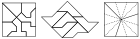
\includegraphics[width=13cm]{images/fig-cuts}
	\caption{Решение пунктов A, B, C}
\end{figure}
}

\section[Нетривиальный счёт]{Nontrivial Count}
\fram{«Средние арифметические», пункт C}{
\begin{block}{Условие}
	Разбить набор $51 \ldots 130$ на четыре поднабора так, чтобы минимум средних был наибольшим.
\end{block}
\pause\medskip\noindent Среднее всех средних неизменно:
\vspace{-0.1cm}
	$$\cfrac{\cfrac{a_1 + \ldots + a_{20}}{20}
		+ \cfrac{a_{21} + \ldots + a_{40}}{20} + \ldots}{4} =
			\cfrac{a_1 + \ldots + a_{80}}{80}.$$
\vspace{-0.1cm}\noindent\pause
Хотим сделать так, чтобы минимум был равен ему. Поднаборы для этого можно взять симметричными.}

\fram{«Фургончик», пункт A}{
\begin{block}{Условие}
Длины стен кузова фургона, который строит себе мороженщик Саша, в метрах выражаются двумя различными простыми числами. Eсли удлинить каждую из стен на 1 метр, площадь фургона увеличится на $\SI{15}{\text{м}^2}$. Найдите размеры фургона.
\end{block}\pause
\vspace{-0.35cm}
$$ab+15 = (a+1)(b+1) = ab+a+b+1\scolon$$
\vspace{-0.52cm}
$$a+b=14\scolon$$
\vspace{-0.52cm}
$$a=11\scolon\ \ b=3.$$}

\fram{«Клиренсы», пункт C}{
\begin{block}{Условие}
Автобус с диаметром колёс 1 метр и колёсной базой $10.5$ метров стоит на планете Маленького принца, диаметр которой 20 метров. Каким должен быть дорожный просвет у автобуса, чтобы он не царапал днищем грунт?
\end{block}
\vspace{0.4cm}
\pause\noindent Идея: имеется равносторонний треугольник со стороной $10.5$ метров.
}

\fram{«Клиренсы», пункт C}{
\vspace{-7.5mm}
\begin{figure}
	\includegraphics[width=8.5cm]{images/autobus}
	\vspace{-1mm}\caption{Отмеченный треугольник — равносторонний.}
\end{figure} \vspace{-2mm}
$$\left( 10 - 10.5 \cdot \frac{\sqrt{3}}{2} \right) + 0.5 = 10.5 \cdot \left( 1 - \frac{\sqrt{3}}{2} \right).$$
}

\section[Игры]{Games}
\fram{«Игры», пункты A, C}{
\begin{figure}
	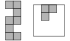
\includegraphics[height=2.5cm]{images/games}
	\caption{Задача «Игры»}
\end{figure} \vspace{-0.6cm}
\begin{itemize}
\item[\bf A.] Первый ставит свою фигуру в центр прямоугольника (ширина же чётная), дальше ходит симметрично\scolon
\item[\bf C.] Первый ставит фигуру как на рисунке. После любого хода второго (из четырёх возможных) ходит так, что второй больше не может походить (перебор).
\end{itemize}
}


\section[Задачи и теория]{Theoretical}
\fram{«Рукопожатия», пункт C}{
\begin{block}{Условие}
Известно, что в Авиаландии пять городов. Из каждого города летает шесть авиарейсов, внутренних или международных. Докажите, что за границы Авиаландии летает чётное количество авиарейсов.
\end{block}
\vspace{0.4cm} \pause
\noindent Всего 30 рейсов\scolon давайте выкидывать внутренние. Каждый внутренний летает между двумя городами, поэтому считается дважды. $30 - \text{чётное}$ — чётное число.
\medskip\noindent Верен и чуть более общий результат.}

\fram{«Как провожают транспортёры», пункт B}{
\begin{block}{Условие}
Два кубика размером $5 \times 5 \times 5$ см едут по транспортёру, причём расстояние между ними равняется 10 см. С данного транспортёра они попадают на следующий, в два раза более быстрый, и дальше едут по нему. Каково расстояние между ними теперь?
\end{block} \pause
\vspace{-0.25cm}$$(5 + 10) \cdot 2 - 5 = 25\ \text{сантиметров}.$$
}

\fram{«Сетки на плоскости», пункт C}{
\vspace{0.3cm}
\begin{block}{Условие}
	Доказать, что любым четырёхугольником можно замостить плоскость.
\end{block}\pause
\vspace{-0.3cm}
\begin{figure}
	\includegraphics[height=3cm]{images/quadr-tessellate.png}
	\caption{Если совместить все вершины четырёхугольника в одной точке — они как раз прекрасно сложатся.}
\end{figure}
}


\section[Конец]{Fin}
\renewcommand{\thefootnote}{/*\!/}
\begin{frame}
	\ \\
	\centerline{\huge Спасибо за внимание!\,\footnote{\ Вы можете задать ещё вопросов}}
\end{frame}
\end{document}
